\documentclass[12pt]{article}
\usepackage{tikz}
\usepackage{pgfplots}

\pgfplotsset{width=7cm}

\begin{document}

Text \tikz[remember picture] \node[circle,fill=red!50] (n1) {}; text.
\vspace{1in}

\pgfplotsset{domain=-1:1}
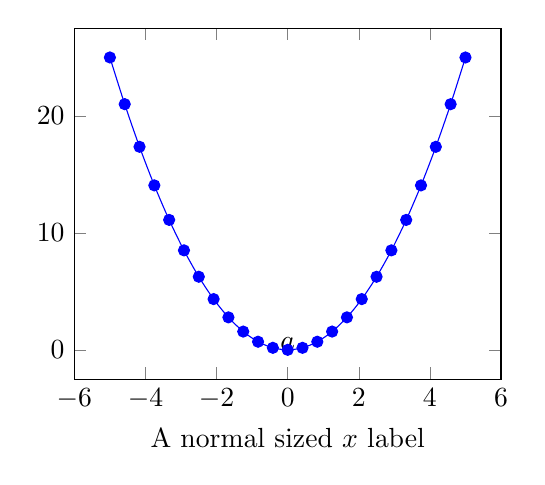
\begin{tikzpicture}
  \begin{axis}[remember picture,xlabel=A normal sized $x$ label]
    \addplot[smooth,blue,mark=*] {x^2};
    \node (c) at (axis cs:0,0.5) {$a$};
  \end{axis}
\end{tikzpicture}
\vspace{1in}

Text \tikz[remember picture] \node[fill=blue!50] (n2) {}; text.

\begin{tikzpicture}[remember picture,overlay]
  \draw [->,red,very thick] (n1) -- (n2);
  \draw [overlay,->,very thick] (c) -- (n2);
\end{tikzpicture}

\end{document}
